\chapter{Plant Fossils and the Story They Tell}%
\label{ch:plantfossils}

In the preceding chapters we have considered the present day plants and plant communities of New Zealand in some detail and those of some other lands more briefly.
Some readers may now wonder how the present botanical patterns developed over geological time and in particular how such widely separated places within and bordering the South Pacific came to have related plants in similar communities.
This is a difficult question to answer, but with plant fossils we do have a sort of time machine, even though the information it provides is very incomplete and sometimes difficult to interpret.
Trying to reconstruct the botany of the past with fossils is a bit like trying to put together large and complex jigsaw puzzles, when many of the parts are missing and some of those we have are difficult, perhaps impossible, to place.
Nevertheless it is often possible to find and correctly fit a sufficient number of pieces to gain at least a general impression of the overall pattern and a very clear idea of some details.

\section{How Do Plants Become Fossils?}

\subsection{Macrofossils}

First of all it is usually detached bits of plants rather than whole plants that become fossils, and this of course makes identification more difficult.
Of macrofossils (visible to the naked eye) the most common are leaves, which often detach cleanly from stems along a special layer of weak cells, then twigs, and, less commonly, cones of conifers and fruits and seeds of flowering plants.
Unfortunately flowers, which are the most reliable means of identification, are mostly soft tissued and often decay before they can become fossils.

Fossilisation frequently takes place at sites in the lowlands where there is deposition of the products of the weathering and erosion of rocks --- clay, silt, sand, and so on.
Such sites are the estuaries and deltas of rivers, river flood plains, ponds and lakes.
Plant parts fall, blow or are washed into these bodies of water, sink to the bottom and become buried under layers of sediment.
As the sediments become deeper and deeper the lower layers are compressed by the weight of those above, they undergo physical and chemical changes and eventually become solid rock.
Any fossils also become greatly compressed and so altered that often all that is left is a carbonaceous film with no cell structure at all.
Such fossils are termed compressions\figureref{\fullref{fig:121fossil-leaf}} and can be revealed by splitting sedimentary rocks along their bedding planes.
\begin{SCfigure}[1.5][!b]
	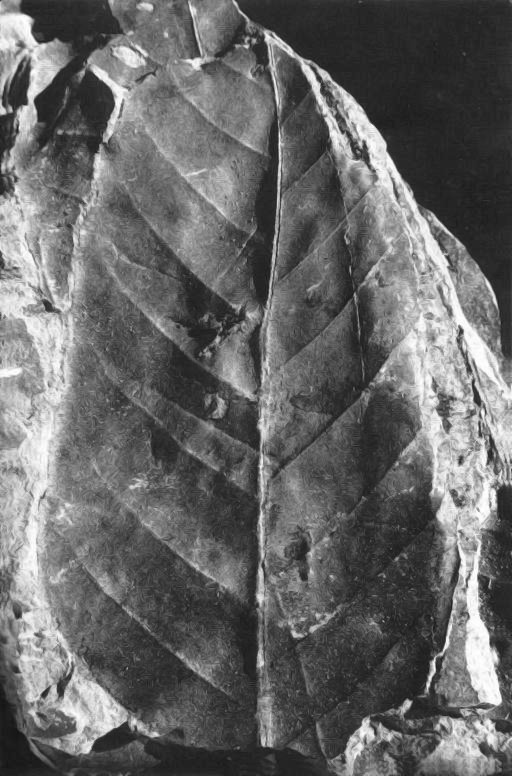
\includegraphics[width=0.4\textwidth]{graphics/fig_121}
	\centering
	\caption[Fossil leaf compression]{Fossil leaf compression about \SI{7}{\centi\metre}$\times$\SI{4}{\centi\metre}, of the extinct \BotanicRef{Nothofagus oliveri}[Nothofagus][oliveri], from Nuggety creek, near Murchison.
	Mid-Miocene age.
	Photo: J. E. Casey.}%
	\label{fig:121fossil-leaf}
\end{SCfigure}
Sometimes there is no original or even substituted plant material remaining, but there may still be an imprint of the plant part.
Such fossil imprints are known as impressions.
Compressions and impressions, particularly of leaves, can reveal a great deal --- shape, margin form and sometimes complete detail of vein systems.
If the resistant waxy surface layers of leaves (known as cuticles) are preserved, the impressions on them of long gone epidermal cells can be studied and their distinctive shapes and arrangements determined.
Sometimes with three dimensional plant parts, such as portions of trunks or branches, the specimen may rot away completely, while the surrounding sediment solidifies, leaving a cavity lined with an impression of its surface.
If the cavity later becomes filled with sediment, this in time solidifies into a cast or replica of the original.

The slow but steady accumulation of organic material in swamps and bogs can also lead to the formation of fossils as the conditions at such sites are often acidic and inhibit decay organisms.
The plant remains, which form peat below the living plants at the surface, are termed subfossils.
If peat becomes deeply buried, particularly under layers of inorganic sediments, pgit ressure and heat gradually convert it into coal and the plant parts steadily lose their structure until none remains in the highest grade coals.

Plants may also be fossilised in fine textured volcanic ash redistributed by the heavy rain often associated with eruptions.

Sometimes the complete cellular structure of fossils is preserved.
This happens when plant material, most often in swamps, becomes impregnated and replaced by silicates (sometimes near silica springs), carbonates and similar compounds in solution.
After such an event the replaced plant material becomes resistant to physical and chemical change and the preservation of cells and sometimes cell contents can be remarkably good even in fossils hundreds of millions of years old.
By special techniques thin sections can be made of these well preserved fossils and cell structure can be studied in detail.

\subsection{Microfossils}

These are principally the spores of ferns, bryophytes and other groups and the pollen grains\figureref{\fullref{fig:122pollen}} of conifers and flowering plants.
\begin{SCfigure}[2.0][!b]
	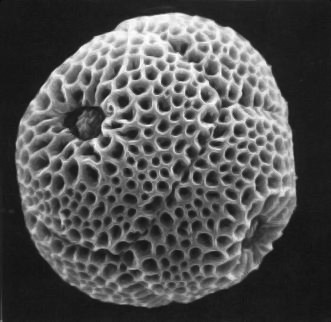
\includegraphics[width=0.4\textwidth]{graphics/fig_122}
	\centering
	\caption[Pollen of \emph{Zygogynum baillonii} of New Caledonia]{Pollen of \BotanicRef{Zygogynum baillonii}[Zygogynum][baillonii] of New Caledonia.
	\BotanicRef{Zygogynum} belongs to the primitive family Winteraceae and at the present day is restricted to New Caledonia.
	The distincative fossil pollen of this or a related genus has been found in New Zelands, in a fossil assemblage of Middle Pliocene Age.
	Photo: F. B. Sampson.}%
	\label{fig:122pollen}
\end{SCfigure}
They are useful in interpreting past floras because of their great resistance to decay (with some exceptions), and because of a number of distinctive and constant characteristics which often enable them to be identified to family, genus or, less often, species.
The resistance to decay derives from a wax-like compound in the cell walls.
The features useful in identification are the shape of the grain (spherical, triangular, bean-like etc); the number, form and arrangement of germination pores; the structure of the wall; and the sometimes intricate pattern of sculpturing on the surface of the spore or grain.

Some plants are more likely to be fossilised than others.
Lowland plants are better represented than alpine plants because it is in the lowlands that deposition is prevalent.
The fossilisation process may begin in suitable alpine sites such as bogs and ponds, but it is likely to be interrupted by erosion at an early stage.
Firm or even hard textured plant parts make better fossils than delicate parts that tend to shred or decay rapidly.
Plant parts which separate readily, such as leaves with abscission layers, are more common as fossils than parts which normally remain attached and slowly decay.
Spores and pollen which are wind dispersed are produced in great quantities and spread for great distances, so are often over-represented in the fossil record by comparison with bird, water or insect-pollinated species.

\section{Lady Lake}

An interesting study was recently carried out at the small Lady Lake in north Westland, New Zealand, in which the relative representation of potential macro-fossils\footnote{\cite{drake1980influx}} and micro-fossils\footnote{\cite{pocknall1980modern}} in the lake sediments was compared with the representation of the present day flora in the region.
Surrounding the lake is \IDX{kahikatea} (\BotanicRef{Dacrycarpus}) swamp forest, conifer broadleaf forest and swamp.
With potential macro-fossils it was found that most trees and shrubs were represented.
Exceptions were \IDX{putaputaweta} (\BotanicRef{Carpodetus serratus}[Carpodetus][serratus]), \IDX{kotukutuku} (\BotanicRef{Fuchsia excorticata}[Fuchsia][excorticata]), \IDX{kaikomako} (\BotanicRef{Pennantia corymbosa}[Pennantia][corymbosa]), \IDX{makomako} (\BotanicRef{Aristotelia serrata}[Aristotelia][serrata], \IDX{wineberry}) and \IDX{hukihuki} (\BotanicRef{Coprosma tenuicaulis}[Coprosma][tenuicaulis]), which all have leaves that decay readily.
\IDX{Kahikatea}[kahikatea] was under-represented and there seems no obvious explanation for this.
Some trees and shrubs appeared to be better represented in the lake sediments than in the surrounding forest --- \IDX{matai} (\BotanicRef{Prumnopitys taxifolia}[Prumnopitys][taxifolia]), \IDX{Hall's totara}[totara!Hall's] (\BotanicRef{Podocarpus hallii}[Podocarpus][hallii]), \BotanicRef{Phyllocladus aspleniifolius}[Phyllocladus][aspleniifolius], \IDX{manuka} (\BotanicRef{Leptospermum scoparium}[Leptospermum][scoparium]), \IDX{kanuka} (\BotanicRef{Kunzea ericoides}[Kunzea][ericoides]), \IDX{southern rata} (\BotanicRef{Metrosideros umbellata}[Metrosideros][umbellata]) and \IDX{mingimingi} (\BotanicRef{Coprosma propinqua}[Coprosma][propinqua]).
Forest floor herbs were not represented in the lake sediments although some high herbaceous epiphytes, \IDX{clubmoss} (\BotanicRef{Lycopodium varium}[Lycopodium][varium]) and the orchids \BotanicRef{Earina} and \BotanicRef{Dendrobium} were.
This may be because the latter are better situated to fall or to be blown into the lake.

Aquatic and swamp species were poorly represented in the lake litter.
Many of them are soft-tissued and decay readily and in the cases of those that are very fibrous, such as \IDX{harakeke} (\BotanicRef{Phormium tenax}[Phormium][tenax]), dead leaves remain attached to the plants and gradually decay.

Some of the litter would be brought into the lake by streams, especially when in flood, some by surface wash during heavy rain, some by direct fall from overhanging plants and some by wind, particularly during gales.

Spores and pollen were sampled from the surface of the lake sediments and from moss cushions.
They gave a picture broadly similar to that of the macro-plant remains, but there were some differences.
By contrast with the lake litter, \BotanicRef{Quintinia}, \IDX{katote} (\BotanicRef{Cyathea smithii}[Cyathea][smithii]) and \IDX{kamahi} (\BotanicRef{Weinmannia}) were under-represented.
The epiphytic orchids were not recorded at all.
The two types of remains were in agreement in under-representing \BotanicRef{Dacrycarpus} and sedges.
It has been suggested that at least some of the under-representation of these species may be due to the rapid decay of their spores or pollen under lake conditions.
Some of these species are well represented in peat where the acid conditions would aid their preservation.

\section{The Fossil Record of New Zealand and Other Southern Lands}
Despite problems of under, over or lack of representation, difficulties in identification due to incomplete and sometimes imperfect preservation, or to some of the fossils being of extinct plants with no modern relatives, it is possible to derive a general picture of the sequence of past botanical events in New Zealand and some related floras.
Before we attempt to do this, however, it is necessary to review the ways in which the positions of crustal blocks in the South Pacific have changed over time,\footnote{\cite{kemp1978tertiary}}\footnote{\cite{crook1981break}} as this is critical to the interpretation of the botanical trends.

\subsection{Crustal Movements}

The modern floras are dominated by flowering plants with conifer and fern components, so we can begin our journey from the past at the time when flowering plants first began to achieve prominence --- the middle of the Cretaceous period\figureref{\fullref{fig:123timescale}} about 100 million years ago.
\begin{figure}[t]
	\centering
	
\includegraphics[width=\textwidth]{graphics/fig_123}
	\caption[Geological time scale]{Geological time scale.}%
	\label{fig:123timescale}
\end{figure}
By this time Africa and India had long since separated from the great southern continent, Gondwana, but Australia, Antarctica and the New Zealand-New Caledonia crustal complex (Tasmantis) were still united\figureref{\fullref{fig:3gondwana}}.
The southern end of South America was probably joined with Antarctica at this stage and remained so until the Oligocene, 30 million years ago.

During the middle Cretaceous, the Australasian portion of Gondwana lay in higher southern latitudes with the northern parts of New Zealand and Australia at about \ang{60}S and \ang{45}S respectively.

In the late Cretaceous (80 million years ago) the New Zealand crustal block began to separate from Australia and Antarctica, moving like a hinge with the northern end of the Lord Howe Rise remaining adjacent to Australia.
By the middle Paleocene (60 million years ago) northern New Zealand had reached \ang{55}S and the Norfolk Ridge had separated from the Lord Howe Rise.
It is possible that there were dry land connections at this time with Queensland, via the Lord Howe Rise, and New Caledonia via the Norfolk Ridge.

In the late Paleocene at about 50 million years ago Australia and Antarctica were moving apart with north Australia reaching \ang{30}S.
Northern New Zealand had attained \ang{40}S by this time.
One result of these crustal movements was the formation of the Lau and Tonga volcanic ridges near to and beyond the northern Norfolk Ridge.
Fiji lay at the northern end of these ridges.

By the late Eocene at 38 million years ago Australia had not changed much in position.
New Zealand had moved further north to approach its present northernmost position of \ang{35}S and the Lau and Tonga ridges had moved eastwards away from the Norfolk Ridge.

The late Oligocene (29 million years ago) saw north Australia reaching \ang{25}S and the activation of the Alpine Fault in the New Zealand region with movement southwards along it of most of the present South Island and the Campbell Plateau and Chatham Rise.
By this time, most of the New Zealand-New Caledonia crustal block was submerged.

By the Late Miocene (10 million years) north Australia was at \ang{15}S and the rearrangement of the New Zealand region along the alpine fault continued.
Between this time and the present the current configuration was attained with north Australia reaching \ang{10}S and New Guinea almost reaching the equator.
In the last few million years crustal movements have raised the New Zealand and New Guinea mountains.

\section{Botanical History}

\subsection{Cretaceous}

The fossil floras of New Guinea, New Caledonia and other smaller islands are too fragmentary and/or poorly known to provide any coherent picture.
Australia, New Zealand, Antarctica and southern South America will be considered together for the Cretaceous period,\footnote{\cite{mildenhall1980new}}\footnote{\cite{wace1965vascular}}\footnote{\cite{dettmann1981cretaceous}} when they were still joined and shared a largely common flora.
For the periods of the Tertiary era, when they had separated and their floras had undergone different trends, they will be treated individually.

In the middle Cretaceous when Australasia, Antarctica and southern South America were joined in high southern latitudes their climates appear to have been much warmer than those of similar latitudes today.
The linked lands also seem to have been generally moist, even in parts now arid, and they shared a type of forest dominated by conifers and ferns with an increasing flowering plant component.
The tree fern family Cyatheaceae was prominent and among conifers the Araucariaceae\footnote{The family Araucariaceae is still represented in New Zealand but with only one species, \IDX{kauri} (\BotanicRef{Agathis australis}[Agathis][australis]). Macrofossils of Araucaria have also been discovered, but as pollen of this genus and Agathis is very similar it is unclear when Araucaria became extinct in New Zealand.} were represented and the Podocarpaceae were becoming dominant.
The earliest flowering plants are known mostly from pollen that cannot be matched with any present day types.

In the latest Cretaceous, when this part of Gondwana began to break up, flowering plants increased in the southern lands and a number of the micro-fossils and macro-fossils can be assigned to modern families, or in some cases genera.
\BotanicRef{Nothofagus} is a notable case with \emph{brassii} group pollen appearing at about the same time in Australia, New Zealand and Antarctica (from fossil pollen near McMurdo Sound) and somewhat later in South America where it was associated with the \emph{fusca} and \emph{menziesii} groups.
Pollen from these two groups appears in New Zealand at the end of the Cretaceous and in Australia in the early Tertiary.
Pollen assignable to the Proteaceae is also found in the four regions in the Late Cretaceous.
In South America, New Zealand, and Australia in particular, a number of other angiosperm fossils of late Cretaceous age have been found but these have not yet been identified.
Some of the families that have been recognised, however, include the Winteraceae, Epacridaceae, Chloranthaceae (\BotanicRef{Ascarina}), Loranthaceae (mistletoes), (?) Scrophulariaceae, Lauraceae, and, rather surprisingly, several families which are largely herbaceous at present, although they may not have been so then --- Ranunculaceae, Haloragaceae (\BotanicRef{Gunnera}), Cruciferae and Caryophyl-laceae.\footnote{\cite{mildenhall1980new}}

\subsection[Tertiary Australia]{Tertiary Australia\thinspace\footnote{\cite{kemp1978tertiary}}\footnote{\cite{martin1981tertiary}}\footnote{\cite{smith1982history}}}

For most of the Paleocene Australia was still joined to Antarctica although a rift valley was developing between them.
Southern Australia was at \ang{65}S but there is evidence that sea temperatures were of subtropical warmth so temperatures on land were probably warm also.
Microfossils indicate widespread forests dominated by Podocarpaceae; \BotanicRef{Nothofagus} was rare.
Araucariaceae, Proteaceae, and Myrtaceae were also represented and in addition \BotanicRef{Anacolosa} and possibly \BotanicRef{Cupania}, genera now restricted to the tropics.
Forests of this type were also present in Central Australia so the general climate was moist as well as warm.
High rainfall, warm temperatures and low relief at this and later times resulted in many places in intensely leached infertile soils which have persisted to the present day.

At the beginning of the Eocene, final separation of Australia and Antarctica began.
At first conditions continued to be warm and moist and further tropical genera were added to the forests such as \BotanicRef{Bombax} (the kapoc genus), and the tropical mangrove palm \BotanicRef{Nipa}.
Conifers and \BotanicRef{Nothofagus} were still poorly represented.
From the middle Eocene the climate cooled, a number of the tropical genera disappeared from southern Australia, and pollen of \BotanicRef{Nothofagus brassii}[Nothofagus][brassii] group increased in importance.

During the Oligocene the climate cooled further and the sparse fossil record indicates similar floras to the late Eocene although with some reduction in diversity.
It is suggested that with the lower temperatures the climates would also have been drier and perhaps relatively arid in northern parts.
An ice cap probably began to develop in Antarctica at this time.\footnote{\cite{kemp1978tertiary}}

In the early Miocene the climate became distinctly warmer and moister than it was in the Oligocene.
The fossils suggest extensive moist forests over southern Australia with \BotanicRef{Nothofagus} of the brassii group, conifers, Myrtaceae and Lauraceae prominent.
In central Australia, localised forests of the same type occurred but so did open habitats as indicated by the record of \BotanicRef{Acacia}, \BotanicRef{Casuarina} and grasses.
Temperatures dropped again by the late Miocene when Australia had reached its present latitudes and the Antarctic ice sheet had reached its present dimensions.
The rather limited evidence\footnote{\cite{kemp1978tertiary}} suggests a retreat of rain forest with the cooler and drier climates.

The Pliocene also began with a warmer phase resulting in some rain forest expansion, but eventually the temperature declined leading to the severe glacial/interglacial oscillations of the Pleistocene.
This finally led to the widespread disappearance of rain forest and expansion of plants adapted to arid conditions.
These included \BotanicRef{Eucalyptus}, \BotanicRef{Casuarina}, \BotanicRef{Acacia} and various Proteaceae.
Most of the arid and semi-arid floral components in Australia are thought to be derived from families of early rain forest origin adapted to heavily leached infertile soils during the Tertiary.

\subsection[Tertiary Antarctica]{Tertiary Antarctica\thinspace\footnote{\cite{wace1965vascular}}}

A site near McMurdo Sound (presently at \ang{78}S) yielded a Cretaceous flora of Podocarpaceae, \BotanicRef{Nothofagus} and Proteaceae.
Palm pollen is recorded in early Tertiary strata from the same locality, indicating a relatively mild climate, even though the latitude was much the same as the present day.
The richest fossil floras of Antarctica are from Seymour Island, off the Antarctic Peninsula at \ang{64}S, where leaves and pollen have been recovered.
The date of these deposits is not certain, but it seems likely to be lower Tertiary.
The flora is reasonably diverse and of rain forest character, although 23 species cannot be identified and of the remainder 27 are ferns including Cyatheaceae and Schizaeaceae.
There is a strong conifer component including the genera \BotanicRef{Araucaria}, \BotanicRef{Agathis}, \BotanicRef{Dacrydium}, \BotanicRef{Phyllocladus} and \BotanicRef{Podocarpus}.
Angiosperms include \BotanicRef{Nothofagus} of the \emph{fusca} and \emph{brassii} groups and the following families: Cunoniaceae, Lauraceae, Monimiaceae (\BotanicRef{Laurelia}), Myrtaceae, Proteaceae (\BotanicRef{Knightia}), Winteraceae, Loranthaceae, Leguminosae, Aquifoliaceae (includes \BotanicRef{Ilex}, the holly genus), Cruciferae and Cyperaceae (sedges).
This assemblage is similar to that produced by the rain forests of Australia in the early Tertiary with the difference that there are no `tropical' taxa, such as \BotanicRef{Anacolosa} and \BotanicRef{Cupania}.

The most recent record of vegetation in Antarctica comes from pollen in Ross Sea deposits of the late Oligocene age.
At this stage an ice sheet was beginning to form.
The assemblages were dominated by \BotanicRef{Nothofagus} pollen (with the \emph{fusca} group most common) plus lesser amounts of Proteaceae, Myrtaceae and Podocarpaceae.

\subsection[Tertiary South America]{Tertiary South America\thinspace\footnote{\cite{wace1965vascular}}\footnote{\cite{kemp1978tertiary}}}

The general progression in South America seems to have been similar to that of Australia although arid climates, while strongly developed in places, did not become so widespread as in Australia.

In the Eocene, genera and families now largely restricted to tropical northern South America appeared in the fossil records of Chile and Argentina.
This is comparable to the appearance of a tropical element in the southern Australian floras at about the same time.
Similarly, with cooling from the Oligocene on, the tropical element disappeared from southern South America and southern rain forest groups --- Podocarpaceae, \BotanicRef{Nothofagus}, Proteaceae, Cunoniaceae --- became increasingly important.

\subsection[Tertiary New Zealand]{Tertiary New Zealand\thinspace\footnote{\cite{mildenhall1980new}}\footnote{\cite{fleming1979geological}}\footnote{\cite{mildenhall1984palaeobotanical}}\footnote{\cite{pocknall1984late}}}

Mountains were raised in the New Zealand crustal complex (Rangitata orogeny) in the late Jurassic and early Cretaceous when it was still part of Gondwana.
By the late Cretaceous, when separation of New Zealand from Gondwana began, it is believed the mountains had been largely eroded, so the physical background to most of the Tertiary fossil record we are about to consider is one of a low lying peneplain with strongly oceanic climates.

During the Paleocene, conifers of the family Podocarpaceae were dominant and \BotanicRef{Nothofagus} of all three groups was fairly rare.
Proteaceae were quite common and, as in Australia, \BotanicRef{Anacolosa} appeared as well as a number of palms including probable \BotanicRef{Nipa Casuarina}[Nipa][Casuarina] also appeared and remained a significant element for most of the Tertiary.
\BotanicRef{Casuarina} no longer occurs in New Zealand as a native genus, but fossil pollen considered to be \BotanicRef{Casuarina} had been known for some time.
The recent discovery of impressions of the distinctive cone-like fruits of \BotanicRef{Casuarina} and the related genus \BotanicRef{Gymnostoma} has confirmed the presence of the family in New Zealand.\footnote{\cite{campbell1985megafossils}}
The Myrtaceae also appear for the first time in the Paleocene with pollen referable to both \BotanicRef{Leptospermum} and \BotanicRef{Metrosideros} having been identified.

In the Eocene the podocarps declined in importance, although \BotanicRef{Phyllocladus} is recorded for the first time.
\BotanicRef{Nothofagus} became dominant, firstly the \emph{fusca} group and latterly the \emph{brassii} group.
\BotanicRef{Cupania} and \BotanicRef{Bombax} appeared, rather later than in Australia, along with a number of new proteaceous genera and \BotanicRef{Freycinetia}, \BotanicRef{Astelia}, \BotanicRef{Quintinia}, possibly \BotanicRef{Phormium}, and the family Araliaceae (includes \BotanicRef{Pseudopanax}).
A genus now extinct in New Zealand, \BotanicRef{Ilex} (which includes the holly), is also first recorded in the Eocene.
Cooling at the end of the Eocene may have been the reason for the extinction of \BotanicRef{Anacolosa}, \BotanicRef{Nipa} and a number of Proteaceae.

During the Oligocene, New Zealand reached its present latitudes and also suffered its greatest reduction in area as a result of sea encroachment.
The cooler climate of the late Eocene seems to have continued into the Oligocene, perhaps partly due in New Zealand's case to the development of cooler westerly winds and currents following the separation of Australia and Antarctica.
The forests were dominated by the \BotanicRef{Nothofagus brassii}[Nothofagus][brassii] group, although the \BotanicRef{Nothofagus fusca}[Nothofagus][fusca] group, \BotanicRef{Casuarina}, \BotanicRef{Myrtaceae}, \BotanicRef{Palmae} and \BotanicRef{Podocarpaceae} were also prominent.
Among genera to first appear in this period are \BotanicRef{Weinmannia}, \BotanicRef{Elaeocarpus}, \BotanicRef{Myrsine}, \BotanicRef{Fuchsia}, \BotanicRef{Coprosma}, \BotanicRef{Laurelia} and \BotanicRef{Epilobium}.

The Compositae (daisy family) made its first appearance in the late Oligocene.

Warmer climates prevailed in the early Miocene and the land began to rise.
Swampy areas were common and surrounding them were dense floristically rich forests.
Many of the species cannot be identified with modern plants, but several \BotanicRef{Nothofagus brassii}[Nothofagus][brassii] group species were common together with Myrtaceae (possibly including \BotanicRef{Eucalyptus}), \BotanicRef{Casuarina}, Podocarpaceae and tree ferns.
Palms also were common and included a small fruited species of coconut in the northern North Island --- \BotanicRef{Cocos zeylanica}[Cocos][zeylanica]\figureref{\fullref{fig:124fossil-coconuts}}.
\begin{SCfigure}[1.0][!b]
	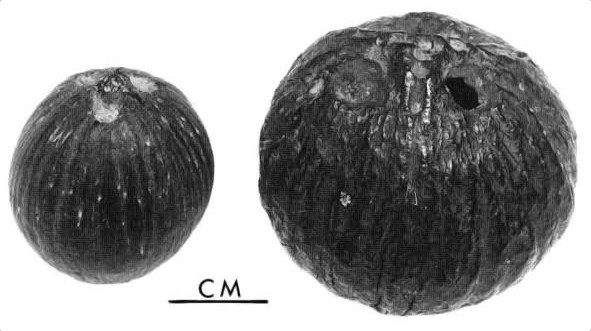
\includegraphics[width=0.5\textwidth]{graphics/fig_124}
	\centering
	\caption[Two fossil coconuts]{Two fossil coconuts of the extinct \BotanicRef{Cocos zeylanica}[Cocos][zeylanica].
	The larger of the two nuts is only about \SI{4}{\centi\metre} across.
	The fossils are associated with a coal seam of Miocene Age at Cooper's Beach in the far north of the North Island.
	The coal seam dips below the sea and the small coconuts are washed onto the beach from time to time.
	Photo: J. E. Casey.}%
	\label{fig:124fossil-coconuts}
\end{SCfigure}
Among genera recorded for the first time are: \BotanicRef{Cordyline}, \BotanicRef{Ripogonum}, \BotanicRef{Dysoxylum}, \BotanicRef{Alectryon}, \BotanicRef{Macropiper}, \BotanicRef{Pittosporum}, \BotanicRef{Muehlenbeckia} and \BotanicRef{Melicytus}.
An interesting incomer is \BotanicRef{Acacia}, no longer present in New Zealand.

Temperatures declined towards the end of the Miocene and this trend continued into the Pliocene.
Uplift continued during the Pliocene and the Southern Alps and other ranges were formed.
This phase of uplift is known as the Kaikoura orogeny and continues today.
Extensive development of alpine vegetation, as we have discussed earlier, would have commenced from this time.
In the lowlands the \BotanicRef{Nothofagus brassii}[Nothofagus][brassii] group was prominent in the early Pliocene but only in the northern North Island.
South of there Myrtaceae, \IDX{rimu} (\BotanicRef{Dacrydium cupressinum}[Dacrydium][cupressinum]), \IDX{red beech} (\BotanicRef{Nothofagus fusca}[Nothofagus][fusca]) group and ferns were common.
By the end of the Pliocene a number of forest genera and species had become extinct including most of the \BotanicRef{Nothofagus brassii}[Nothofagus][brassii] group, \BotanicRef{Bombax}, \BotanicRef{Cupania} and many palms.

During the Pleistocene the climate deteriorated greatly with a succession of long glacials and shorter interglacials.
The last species of the \BotanicRef{Nothofagus brassii}[Nothofagus][brassii] group disappeared together with \BotanicRef{Microstrobus} and \BotanicRef{Microcachrys} (now restricted to Australia) of the Podocarpaceae, \BotanicRef{Casuarina}, (?) \BotanicRef{Eucalyptus}, \BotanicRef{Acacia} and all Proteaceae except two species, namely \IDX{rewarewa} (\BotanicRef{Knightia excelsa}[Knightia][excelsa]) and \IDX{toru} (\BotanicRef{Toronia toru}[Toronia][toru]).
With each glacial the alpine vegetation expanded and diversified; with each interglacial the forests expanded from refugia (albeit reduced in diversity) to largely reclothe the landscape.

\section{Disjunct Distribution Patterns}

Certain present day anomalies in the distribution patterns of New Zealand species are thought by some to have been caused by these climatic fluctuations.

Wardle\footnote{\cite{wardle1963evolution}} noted that the northern North Island and northern and southern South Island regions have much higher numbers of endemic species (90 to 110) than the southern North Island and central South Island (25 to 30).
The endemics of the northern North Island are mostly woody and lowland and those of the northern and southern South Island mostly herbaceous and alpine.

Wardle also observed that there are a number of species disjunct between the regions of high endemism, for example \IDX{tanekaha} (\BotanicRef{Phyllocladus trichomanoides}[Phyllocladus][trichomanoides]) and \IDX{kauri grass} (\BotanicRef{Astelia trinervia}[Astelia][trinervia]) between the northern regions of the two islands, and \IDX{mountain daisy} (\BotanicRef{Celmisia traversii}[Celmisia][traversii]) and species of \BotanicRef{Nothofagus} between the northern and southern South Island.

It is suggested that these anomalies have the same explanation.
During the last glaciation the central South Island with its high mountains would have been more severely glaciated than the neighbouring regions.
Its flora would have been more reduced with the local extinction of some species that survived to the north and south.
The low endemism of the southern North Island is more difficult to explain, but a somewhat lower treeline at the present time than would be expected and some fossil evidence indicates that climatic conditions were relatively severe there during the last glaciation.

Recently McGlone\footnote{\cite{mcglone1985plant}} has proposed a quite different explanation.
He believes that the causes of these anomalous patterns are tectonic not climatic and must be sought much further back in time in the late Tertiary before the glacial/interglacial fluctuations had commenced.
At this time much of the southern North Island had become submerged beneath the sea and this would explain the low endemism and some of the disjunctions.
In the South Island the uplift of particularly high mountains in the central region would have greatly altered habitats there and:

\begin{quote}
	as a result the once continuous, upland flora was split into northern and southern regions, where the rate of uplift was low and average age of surfaces older, and a rapidly uplifting central zone.
\end{quote}

\section{In Conclusion}

The fate of the original vegetation cover of the various regions of the Australasian/Antarctic portion of Gondwana has depended on crustal movements and climatic change.

In the case of Antarctica, deterioration of the climate in the later Tertiary eventually led to the extinction of vascular plants.

The northward movement of Australia during the Tertiary counter-balanced the temperature decline to some degree, but the pronounced cold spells of the Pleistocene played some part in the disappearance of closed forest from most of the continent.
However the major cause of the drastic vegetational changes from the late Tertiary would have been increasing aridity associated with declining temperatures.
In the southern hemisphere, aridity is most marked along the Tropic of Capricorn which Australia now straddles.

The extent to which the rich rain forests of New Guinea correspond to those which were formerly widespread in Australia is uncertain.
Until recently it was thought that much of New Guinea's rain forest flora was derived from south-east Asia after contact was made with that region.
This was also thought to be the case with the rain forests of north Queensland, but this has recently been questioned as many of the genera concerned have a fossil record in Australia extending back to times when Australia and its northern portion which became New Guinea was still far south of Asia.\footnote{\cite{webb1986recent}}
Certainly the rain forests of New Guinea in near equatorial latitudes would not have been greatly affected by cooler, drier climates during the Pleistocene.
The alpine flora of New Guinea, as already mentioned, although interesting, is not particularly rich and includes Asian and Australasian components.

Botanically speaking, New Caledonia is one of the most interesting fragments of Gondwana.
Being tropical like New Guinea, although not equatorial, with a strongly oceanic climate due to its narrowness, it too has probably not been greatly affected by coolness or drought.
As a consequence its inheritance of Gondwana conifer and angiosperm families would have survived better than those of Australia and New Zealand.
This makes it of special importance to botanists in the latter countries attempting to reconstruct the history of their own floras, as now extinct genera in Australia or New Zealand may still have extant species in New Caledonia.
A special development in New Caledonia has been the evolution of many species, mostly of Gondwana genera, tolerant of the soils of the extensive areas of ultramafic rock.

Finally we come to New Zealand.
Like Australia, New Zealand's northward movement during the early Tertiary would have moderated the effects of any temperature declines and its oceanic climate would have countered any tendency to aridity.
However, New Zealand had attained its present position some time before the more drastic climate deterioration of the Pleistocene and the cold climates deriving from the combined effects of high mountains and glaciations, although ameliorated to some extent by an oceanic climate, greatly affected the vegetation.
Forests retreated and some of their genera and species became extinct, while new species evolved in colder open habitats contributing to the present relatively rich alpine flora.

The native forests include genera with a long history in the region; the plants of the mountains are a more recent burgeoning of specialised forms in response to the uplift of the mountains and episodes of climatic refrigeration.

The recent advent of human habitation has greatly reduced New Zealand's natural cover --- Polynesians achieved it with fire and, to more effect in a shorter time, Europeans with fire, the plough and the introduction of alien plants and animals.

The time has surely come to call a halt, to preserve those areas of largely intact vegetation we still have and to actively encourage the regeneration of native plants in areas abandoned from farming where fire and browsing have taken their toll.
